% This is LLNCS.DOC the documentation file of
% the LaTeX2e class from Springer-Verlag
% for Lecture Notes in Computer Science, version 2.4
\documentclass{llncs}
\usepackage{llncsdoc}
\usepackage{color}
\usepackage{graphicx}
\usepackage{subfigure}
\usepackage{listings}
\usepackage{bold-extra}
\usepackage{wrapfig}
\usepackage{enumerate}
\usepackage{float}
\usepackage{algorithm2e}
\usepackage[backgroundcolor=pink!40]{todonotes}
%



\begin{document}
\lstset{ 
	language = [AspectJ]Java,
  basicstyle=\ttfamily\footnotesize,
  numbers=left,
	numberstyle=\tiny\color[rgb]{0.25,0.25,0.25},
  firstnumber=auto,
	breaklines=true,
  tabsize=2,
	emph={aspect,declare, adapter, instance, pointcut, adaptee, adapts, select, UNTIL,pc,name, instanceType, exp, removeExp}, 
	emphstyle=\textbf,
	stringstyle=\textsf,
	showstringspaces= false,
	frame=single
	}

\title{Instance Pointcuts}
\subtitle{An Aspect-Oriented Mechanism for Maintaining Object Sets}

\author{Kardelen Hatun \and Christoph Bockisch \and Mehmet Ak\c{s}it}
\institute{TRESE, University of Twente \\ 7500AE Enschede \\ The Netherlands \\
\url{http://www.utwente.nl/ewi/trese/}\\
\email{ \{hatunk,c.m.bockisch,aksit\}@ewi.utwente.nl}
}

\maketitle

\begin{abstract}
In the life-cycle of objects there are different phases. The phase in which an object currently is, affects how it is handled in an application; however these phase shifts are typically implicit.
In this study we propose a new language mechanism, called instance pointcuts, based on aspect-orientation.
They maintain sets of objects according to events in their life-cycle and create notifications when new objects are added or removed from the set.
The selection criteria of instance pointcuts can be refined, e.g., to define a subset or super-set of an existing instance pointcut; and they can be composed, e.g., by set operations.
Our approach improves modularity by providing a fine-grained mechanism and a declarative syntax to maintain a set of objects.
\end{abstract}

\section{Introduction}
In object-oriented programming (OOP), objects encapsulate state and behavior; objects also have a life-cycle, which means that the same object can play different roles at different times. And which role an object is currently playing is important as it can affect the object's own behavior or how objects are handled. Typically the shift from one life-cycle phase to another is implicit, e.g., determined by passing an object from one client to another. In this paper, we propose a new language mechanism for declaratively specifying life-cycle phases and for exposing the set of objects which are currently in a specific phase. This declarativity allows us to give guarantees about these sets like subset relationships, as well as to perform compile-time checks like warning about sets that will always be empty.

As an example of different relevant phases in the life-cycle of objects, consider an online store application. Assume that the offered products are objects in the program and that specific budget plans should be offered for products depending on their life-cycle phase. A first example of such a phase is a period during which a product is in the wish-list of any customer; this phase begins when ``product'' object is added to the ``wish-list'' property of a ``customer'' object and it ends when it is removed from this property. A second example is the phase when an object is out of stock. Thus, we defined two sets of objects: the set of objects into which at least one customer is interested and the set of objects that are sold out. Finally, the shop owner may be interested in the intersection of these sets and give priority to reordering the corresponding products.

Furthermore, in OOP objects are categorized according to their \emph{types}.
This is a structural categorization and it does not give any information about the events that object participates in.
However, grouping objects according to another criteria such as, the class they were initialized in or being passed as an argument to a certain method would only be possible by inserting code at those particular points, which would litter the code.

To be able to process the objects which are currently in a relevant life-cycle phase (like having been added to a wish-list), bookkeeping is required to keep track of the set. To separate this bookkeeping code from the business logic of the program, aspect-oriented programming (AOP) is a well known technique. But in AOP, \emph{pointcuts} select sets of so-called \emph{join points} which are points in time during the execution of the program; current aspect-oriented languages do not offer dedicated mechanisms for selecting \emph{sets of objects}.

These languages do not support a \emph{declarative specification} of the objects belonging to a life-cycle phases; instead an \emph{imperative implementation}, always following the same pattern, is required for collecting those objects.
A consequence of such an imperative solution, besides all the negative effects of hand-writing boilerplate code, is that automatic reasoning becomes practically impossible.
In addition, a declarative implementation makes the relevant information explicit, which reduces checking efforts as well as making the code readable.

To offer better support for processing objects according to their life-cycle phase, we propose a language construct that builds on the technology of aspect-orientation.
We borrow the terminology and provide \emph{instance pointcuts} to select sets of objects based on the execution history.

An instance pointcut definition consists of three parts: an identifier, a type which is the upper bound for all objects in the selected set, and a specification of relevant objects.
%Instance pointcuts do not have any parameters, the only information that is explicitly given is the \emph{type} of the instance we are interested in selecting.
The specification consists of two \emph{pointcut expressions} that select relevant join points in the objects' life-cycle and expose the object: the mark the beginning and end of a life-cycle phase; i.e., the object is added to or removed from the set.

New instance pointcuts can be derived from existing ones. One instance pointcut can be declared to be a \emph{subset} or a \emph{super-set} of an existing one.
In this case, the specification of the life-cycle phase is narrowed down or broadened, respectively.
%One way is to refer to an instance pointcut and \emph{co-variantly} refine its selected type. Another way is to This composition mechanism is strengthened with the ability to declaratively define a pointcut as a \emph{subset} or a \emph{super-set} of another one. These relationships come with additional checks which ensure that there are no inconsistencies between a super-set and its subsets, such as a subset containing instances that are not members of its super-set.
Composition of existing instance pointcut is also supported in terms of set operations: \emph{intersection}, \emph{union} and \emph{set difference}. 

%, and the exposed variable is added to the set. It is also possible to remove object from the set and this is done via the \emph{de-selection} expression which is also defined in the form of a pointcut expression. When the expression is evaluated to be true, if the exposed instance exists in the set then it is removed. It is possible to point to certain places at join-points via using before and after clauses. With this feature it is possible to select instances before they are passed as an argument or after they call a method. 


\section{Motivation - Example Section}
\label{sect:motivation}

Objects can be categorized by how they are used (passed as arguments to method calls, act as receiver or sender for method calls, etc.). Concerns may be applicable to objects used in the same way. Therefore we must be able to identify and select those objects that are similarly used. Since object behavior is the building block of system behavior, such a categorization will allow behavior extensions on the object-level, providing an extra dimension of modularity.

In the remainder of this section we outline the architecture and design of an online store application. Then we use this scenario to give examples of categorizing objects according to how they are used and how to use these categories in the implementation of some concerns. Finally we conclude requirements from these examples.
\paragraph{Online Shop}
An online shop is a sophisticated web application and objects of the same type can exist at different stages of the control flow. Typically such objects have properties which indicate their \emph{state}. At certain points in execution these states are updated  accordingly. In Figure \ref{fig:shop} the static structure of a simplified online shop is shown. When a new user logs in, \texttt{SessionManager} creates a \texttt{Customer} object to represent the user's session. A customer has a \texttt{ShoppingBag} which may contain arbitrary \emph{items} and a \texttt{WishList} which may contain arbitrary \emph{products} . The class \texttt{Item} represents a concrete \texttt{Product}, e.g. when the user selects a product and clicks add to shopping bag, an \texttt{Item} is added to the \texttt{ShoppingBag} object, aggregating the selected \texttt{Product}. The abstract class \texttt{Product} is super-type of all products in the shop. The \texttt{Product} is further broken down to product categories such as beauty, electronics etc. There are two customer types in the system, \texttt{RegularCustomer} and a \texttt{GoldCustomer}. \texttt{GoldCustomers} can benefit from additional discounts when buying certain products. A customer can add/remove items from his shopping bag. When the shopping is finished then the \texttt{purchase()} method is invoked which returns an object of type \texttt{Order}. To complete the order the customer has to provide payment information (\texttt{PaymentInfo}) and shipping information(\texttt{ShippingInfo}). Once this information is complete the order is finalized. 

\begin{figure}[b]
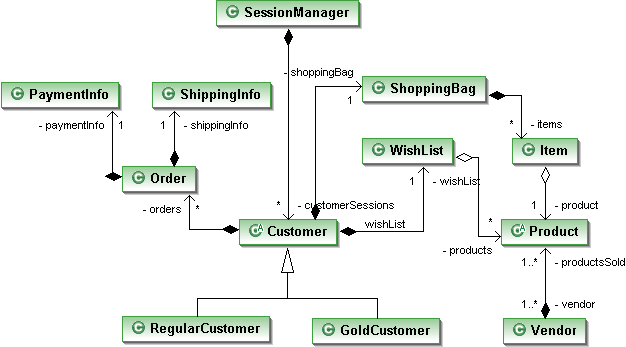
\includegraphics[width=\textwidth]{images/onlineshop_son.png}%
\caption{A simple online shop application}%
\label{fig:shop}%
\end{figure}


\paragraph{A New Requirement}
Let's assume a new requirement for applying more sophisticated discount rules to products is introduced. The rules should should apply to a subset of \texttt{Item}s which are selected when they exist in the context of an interesting event. In order to realize this in an OO-approach, one needs to insert the code regarding the discount concern, to the place where the event of interest occurs. For the following discount rule; \textsf{when an item is added to a shopping bag between certain hours, then they are applied the happy-hour discount}, we need to invasively change the system code by inserting a check for \emph{timing condition} and a method call for applying the discount rule should the condition hold. In Listing \ref{lst:happyhour} the code is inserted in the method \texttt{addtoShoppingBag} of \texttt{Customer} class.

\begin{lstlisting}[caption={A Java implementation of Happy-hour discount rule}, label={lst:happyhour}]
public boolean addToShoppingBag(Product p, int amount)
{
	Item item = ItemFactory.createItem(p,amount);
	/*The discount concern*/
	if('timing condition')
		ProductManager.applyDiscount(item, DiscountRule.getRule(HAPPY_HOUR));
	/*********************/
	this.shoppingBag.add(item);
}
\end{lstlisting}

Even for a single discount rule, the code for the discount concern creates cluttering. If we would like to apply multiple discount rules for the \emph{add to shopping bag} event, this way of implementing is clearly not suitable. Maybe another solution can be changing the method signature of \texttt{addtoShoppingBag} to include a parameter for \texttt{DiscountRule}. However this event may not be the only event we want detect for applying discount rules and the OO implementation will eventually be scattered and tangled. An aspect-oriented implementation can offer a better solution , by encapsulating the concern in an aspect. In Listing \ref{lst:happyhouraop} the \texttt{pc} pointcut selects join-points where customer adds a product to his bag. The advice is executed when \texttt{pc} is matched; after the timing condition is checked the desired discount is applied.

\begin{lstlisting}[caption={An Aspectj implementation of Happy-hour discount rule}, label={lst:happyhouraop}]
pointcut pc(Item item): call(* ItemFactory.createItem(..)) && withincode(* Customer.addToShoppingBag(..));

after() returning(Item item): pc(item)
{
	if('timing condition')
		ProductManager.applyDiscount(item,DiscountRule.getRule(HAPPY_HOUR));
}
\end{lstlisting}

If we make the same discount rule more complex by saying; \textsf{apply a happy-hour discount only to beauty products} then we should insert an \emph{instance of} check to the \texttt{Product} the \texttt{Item} instance holds, to apply the right kind of discount. This situation becomes more complex when there are multiple discount rules, for various types of products. This imperative way of selecting objects becomes error-prone. The aspect implementation, while successfully encapsulating the discount concern, becomes riddled with boilerplate code and it suffers from the same error-prone checks the OO implementation does. Once the happy hour is over, the discount needs to be removed from items. With the current implementation, we do not know which items are applied a discount, because we did not do any book-keeping. In order to remove the discounts, we either have to do a complicated checking regarding the type of the products and when it was added to the shopping bag, or there should be a global structure holding these set of elements, which means adding book-keeping concern to the implementation. 

Instead of creating a new set structure everytime a discount rule is applied, we may want to select a subset of an existing set to apply the discount. For example in a set of \texttt{BeautyProduct}s, we may want to access the subset \texttt{HandCream}s. Java requires we iterate over the set and check each product's type to see if it is of type \texttt{HandCream}. With AspectJ, we can select join-points where an element is put to the beauty products set, and expose the element to check if it is an hand cream. Both of these imperative implementations suffer from boilerplate code and reusing the sets for refinement or other set operations causes makes the code unreadable and error-prone.


\todo[inline]{what needs to change to support them?}
In order to overcome the shortcomings of existing approaches, we need a way to declaratively select objects based their life-cycle phases, where the beginning and the end of a phase is marked by events. From the scenarios described above, we conclude the following requirements:

\begin{enumerate}[{Requirement}1{:}]
\item reifying set of objects, adding/removing object from the set
\item multi-set
\item Events and select objects from the context of the event
\item access the set of objects which is currently selected and be notified when the set changes
\item refinement: subset and support
\item composition: set operations
\item checks: validity of composition, empty sets
\end{enumerate}




%\subsection{Potential Scenarios}
%\begin{enumerate}
	%\item When a product is wish-listed by a GoldCustomer, then apply a discount to it. 
	%\item When products are added to a shopping bag between certain hours, then they are applied the happy-hour discount
	%\item When products are added to GoldCustomer’s shopping bags, apply an additional discount
	%\item When a product is marked low selling by the system, put an advertisement for it on the sidebar → refinement low selling books..., 
	%\item if product is low selling →  notify the vendor
	%\item superset: beauty products, sub-set: beauty products by guerlain which are wishlisted on workdays
	%\item composition:intersect(low selling products && products from Vendor A && products which are lipsticks)
	%\item When it is added to a shopping bag its price may be decreased by applying a discount policy. These examples contain an initial event that is associated with a particular instance, which triggers a follow-up event. 
%\end{enumerate}




\subsection{Explanation of features, just a summary}
Selecting a set of objects based on their life-cycle events provide a new dimension in categorizing objects. Instance pointcuts reify such a set, by offering a declarative syntax for adding objects to it. The object to be added is exposed in the context of the matched event. An object might only be relevant during a particular phase of its life-cycle, which is marked by certain events. Then it is necessary to have a mechanism to remove objects from the set once the event that marks the end of that phase is encountered. Hence, it is possible to declare an optional removal expression in an instance pointcut.

Instance pointcuts represent a set, and the objects in this set can be accessed through instance pointcuts. Also when there's a change in the set, i.e. an object is added or removed, it is  possible for the interested modules to access the change events. 

Sets can have subsets or supersets. This is also true for the sets of objects created by instance pointcuts. An instance pointcut can be refined to obtain the subset of objects it originally selected or it can be a subset of another instance pointcut which broadens its scope. This refinement mechanism makes instance pointcuts reusable. Composition is also supported via the ability to perform set operations on instance pointcuts. It is possible to define intersection or union of two instance pointcuts, in order to define a new one. 

The various features instance pointcuts offer also require some checking to be performed. For example when refining a pointcut to obtain a subset, we may end up with an empty set. This situation should be checked and necessary warning should be given. Since instance pointcuts dedicated to a type, the composition operations may fail if the composed pointcuts do not select co-variant types, which should also be checked.






\hline
\hline

\section{Instance Pointcuts}

Instance pointcut is a declarative language construct that is used to select a set of objects of a specific type. The result of the selection is a \emph{set}, hence it cannot contain the same object more than once. Instance pointcuts provide the ability to select objects over a period marked by events in their life-cycle, modularizing the object selection concern. It also provides a mechanism to construct a set of objects according to relevant events, the places in application those events take place and object state at a certain point in execution. Instance pointcuts lets the user to make focused selections,therefore manage the system at a finer level.In the remainder of this section, we will explain instance pointcuts in detail. 

\todo[inline]{maybe section outline summarizing main features}
\missingfigure{Static Structure of instance pointcuts}

\subsection{Basic Syntax}

A concrete instance pointcut definition consists of a left hand-side and a right-hand side. In the left hand side the pointcut's name and the instance type of interest is declared. Instance pointcuts cannot declare variables, it only has a single implicit variable called \texttt{instance} of the declared instance type. In the right hand side a pointcut expression describes the desired join-points and then binds the exposed object as a member of the instance pointcut's set, which is represented by the variable \texttt{instance}.  It is also possible to declare an abstract instance pointcut, by leaving out the right hand side and placing the \emph{abstract} modifier at the beginning of the declaration.

\begin{lstlisting}[float=h!]
instance pointcut customers<Customer>: call(SessionManager.createCustomer(..)) && returning(instance)
\end{lstlisting}

The instance pointcut above shows a basic example. The left-hand side of the instance pointcut indicates the pointcut is called \texttt{customers} and it is interested in selecting the \texttt{Customer} objects. On the right-hand side, the pointcut expression selects the join-points where \texttt{Customer} is returned by the \texttt{createCustomer} of the class \texttt{SessionManager}. The returned instances are exposed and bound by the \texttt{returning} clause to the \emph{implicit variable} \texttt{instance}, which represents a member of \texttt{customers}' set. After selecting a set of objects, instance pointcuts offer ways to manipulate this set. 




\subsection{Supported AspectJ Predicates}

\todo[inline]{Here we will discuss which predicates we support, with additional explanation of the returning clause}

\subsection{before / after Statements}

\todo[inline]{How to use them and invalid combinations}
\todo[inline]{What is the default behavior if they are not explicitly defined}
\todo[inline, color =green!40]{Additional checks?}
\missingfigure{Example using before after statements}

\subsection{Deselection}

\todo[inline]{How to deselect instances, what are possible checks?}
\missingfigure{Example using UNTIL clause, also incorporating before/after}

\subsection{Instance Pointcut References}

\todo[inline]{how to reference instance pointcuts}
\todo[inline]{Type-refined references}

\subsection{Instance Pointcut Composition}

\subsection{Subsets}

\todo[inline]{Explain what type of relationships subsets stand for}
\todo[inline]{Paragraph: subsetting by type refinement}
\todo[inline]{Paragraph: subsetting by narrowing down the pointcut expression with additional predicates}
\missingfigure{Examples of subsetting, type refinement, additional predicates and both}

\subsection{Supersets}

\todo[inline]{Explain what type of relationships supersets stand for}
\todo[inline]{Paragraph: superset by composing multiple instance pointcuts refer to union operation}
\todo[inline]{Paragraph: superset by composing an instance pointcut with an expression}
\missingfigure{Examples of supersetting}

\subsection{Union, Intersection and Set Difference}
\todo[inline]{Define these operations and give simple examples}


\subsection{Refinement} 
It is possible to refine instance pointcuts in multiple ways. Normally instance pointcuts are referenced by their name, however they can also take an additional statement for \emph{type refinement}, which selects a subset of the instance pointcut dynamically. Type refinements require that, the refined type is a subtype of the original instance type. For example the instance pointcut \texttt{customers} can be refined with the following syntax: \lstinline!customers<GoldCustomer>!. 
This indicates we would like to select the subset of \texttt{GoldCustomer} instances from the set of \texttt{Customer} instances selected by \texttt{customers}. 
Note that this notation will also select subtypes of \texttt{GoldCustomer}. 
If this is not the desired effect then the following: \lstinline!instance pointcut goldCustomers<GoldCustomer>: customers && if(instance.getClass().equals(GoldCustomer.class))! can be used. 
The effect of a refinement subset being empty is equivalent to that of an unmatched pointcut. 
%Note that if the \textbf{+} operator was not used in the pointcut expression, the refinement expression would still be legal, since \texttt{Rectangle} is a subtype of \texttt{Shape}. However it would result in a warning explaining the \texttt{Shape}'s subtypes are not selected.

Instance pointcuts can also be refined inside a pointcut expressions and the refinement result will then be assigned to the instance pointcut on the left-hand side. Once again refining the \texttt{customers} pointcut, we can define the following:

%\vspace{-15}
\begin{lstlisting}[float=h!]
instance pointcut goldCustomers<GoldCustomer>: customers &&  if(instance.getGoldCustomerID().startsWith(``NL''))
\end{lstlisting}
%\vspace{-15}

The \texttt{goldCustomers} instance pointcut is interested in \texttt{GoldCustomer} objects which are selected by \texttt{customers} and who have \texttt{goldCustomerID}s starting with the string ``NL''. The pointcut expression to select these instances is very concise and is shown in the listing above. \texttt{customers<GoldCustomer>} statement selects the \texttt{GoldCustomer} instances selected by \texttt{customers} pointcut, then the \texttt{if} pointcuts checks whether these instances satisfy the condition. Note that the following statement; \lstinline!instance pointcut regularCustomers<RegularCustomer>: customers<GoldCustomer> &&  if(instance.getGoldCustomerID().startsWith(``NL''))! , would result in a compile error for two reasons. First we cannot assign \texttt{GoldCustomer} instances to a \texttt{RegularCustomer} instance pointcut. Secondly \texttt{instance.getGoldCustomerID()} is illegal since \texttt{instance} is the implicit variable of the \texttt{regularCustomers} pointcut and it has the type \texttt{RegularCustomer}, which does not have the property \texttt{goldCustomerID}.

Refinement mechanisms provide a consistent selection process and reduce redundancy. Being able to select subsets of instance pointcuts, eliminates the need for defining separate pointcuts for subsets, which may result in erroneous selections. Since the refinement only supports the subtypes of the original instance type, it works with the system's type hierarchy in a natural manner. 

\subsection{Deselecting Instances}
\label{sec:deselect}
The examples of instance pointcuts presented so far were for selecting objects. Once an object is selected, it does not have to remain in the instance set until it dies. It is possible to define removal conditions in the form of pointcut expressions, that can point to any event in the object's life-cycle.

In the listing below the instance pointcut \texttt{rectangle} selects the subset of \texttt{Rectangle} objects which are selected by \texttt{shapes} pointcut. These instances are selected \emph{until} the pointcut expression that follows the keyword \texttt{UNTIL} is true.

\begin{lstlisting}[float=h!]
instance pointcut rectangle<Rectangle>: shapes<Rectangle> UNTIL call(* Rectangle.setWidth(..)) && if(instance.getWidth() > 10) && target(instance)
\end{lstlisting}

The ability to deselect instances provides flexibility over managing instances. With this mechanism user can select a period in an instance's life-cycle where the beginning and the end of the period is marked by pointcut expressions.

\textbf{\textcolor[rgb]{1,0.41,0.13}{Advice before / after?}}

\subsection{Compilation of Instance Pointcuts}

Instance pointcuts are implemented as an extension to AspectJ, they reuse AspectJ pointcut expressions, however they also allow \texttt{returning} clause in the pointcut expression to capture returned objects. In Figure \ref{fig:ip} static structure of this extension is shown. Both \texttt{InstancePointcut} and \texttt{AspectJPointcut} inherit from the \texttt{Pointcut} abstract class. As seen on the diagram, instance pointcuts can have two pointcut expressions, one is inherited from \texttt{Pointcut} and is called \texttt{exp}. This attribute is also inherited by the AspectJ pointcut. The second one is however specific to instance pointcuts (\texttt{removeExp}) and it can be used to define pointcut expressions for deselecting instances(Section \ref{sec:deselect}). Note that the \texttt{PointcutExpression} class is a subtype of \texttt{ConditionalExpression} \textbf{\textcolor[rgb]{1,0.41,0.13}{(Mention JaMoPP)}}. Another notable difference between AspectJ and instance pointcuts is that AspectJ pointcuts are parametrizable (\texttt{Parametrizable} interface), while instance pointcuts have a single implicit parameter called \emph{instance}. The type of this parameter is stored in the mandatory attribute \texttt{instanceType}.

\begin{figure}
\centering
   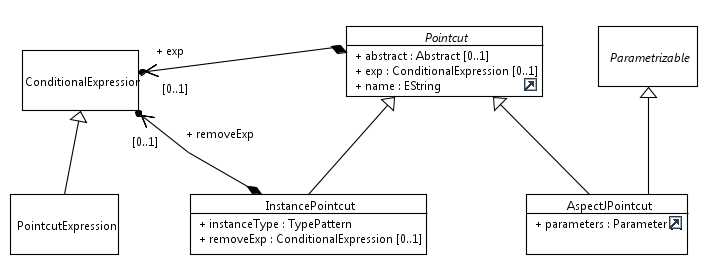
\includegraphics[width=\textwidth] {images/pc.png}
   \label{fig:shapes}
\label{fig:ip}
\caption{Instance pointcut static structure}
\end{figure}

Instance pointcuts can be compiled to various AO-languages, for our prototype we chose AspectJ as the target language. A pseudo-code of the generator template for instance pointcuts is shown in Listing \ref{lst:ip2aj}. 

%\begin{lstlisting}[float=H, caption={Code generation templates for instance pointcut to AspectJ generation }, label={lst:ip2aj}]
%Enumeration ExpressionType {SELECT, REMOVE}
%generate(InstancePointut pc){
	%if(pc.isAbstact){
		%'abstract pointcut' pc.name'('pc.instanceType 'instance)'
		%'Set<'pc.instanceType'>' pc.name'_set'
	%}
	%else{
		%'Set<'pc.instanceType'>' pc.name'_set = new TreeSet<'pc.instanceType'>();'
		%generateAspectJCode(pc, SELECT);
		%if(pc.removeExpression != null)
			%generateAspectJCode(pc, REMOVE);
  %}
%}	
%generateAspectJCode(InstancePointcut pc, ExpressionType eType){
	%String pcname, setOperation, setName = pc.name + '_set';
	%PointcutExpression expTemp;
	%switch(eType){
		%case REMOVE:{
			%pcname = pc.name + '_remove';
			%setOperation = 'remove';
			%expTemp = pc.removeExp;
		%}
		%case SELECT:{
			%pcname = pc.name;
			%setOperation = 'add';
			%expTemp = pc.exp;
		%}
	%}	
	%if(exp.contains(ReturningStatement))	{
		 %PointcutExpression newExp = expTemp.remove(ReturningStatement);	
		%'pointcut' pcname'():' print(newExp) ';'
		%'after() returning(' instanceType 'instance):' pcname'(){'		
	%}
	%else{
		%'pointcut' pcname'('pc.instanceType 'instance):' print(expTemp) ';'
		%'after(' pc.instanceType 'instance):' pcname'(instance){'	
	%}
	%'boolean flag ='setName.setOperation '(instance);
	 %if(flag)
		%print(instance  +' setOperation ');
	%}'
%}
%\end{lstlisting}

\section{Compilation of Instance Pointcuts}
\todo[inline]{AspectJ code generation}
\todo[inline]{Generation of instance pointcut related hooks in the form of aspectj pointcuts, such as add/remove operations to the instance pointcut set}
\missingfigure{compilation algorithm?}

\section{Related Work}
\section{Discussion}
\section{Conclusion and Future Work}
\todo[inline]{keep it short}

\end{document}